\documentclass[a4paper,10pt]{article}
\usepackage[utf8x]{inputenc}
\usepackage[top=1.5cm, bottom=1.5cm,left=2cm,right=1.5cm]{geometry}
\usepackage{url}

%opening
\title{Statistical Analysis of ISMB Coverage at FriendFeed 2008 - 2011}
\author{Neil Saunders}

%load data

%functions

\usepackage{Sweave}
\begin{document}

\maketitle

\begin{abstract}
This document analyses coverage of the ISMB conference at FriendFeed, from 2008 to 2011.
\end{abstract}

\section{Posts, comments and comment/post ratio}

\begin{center}
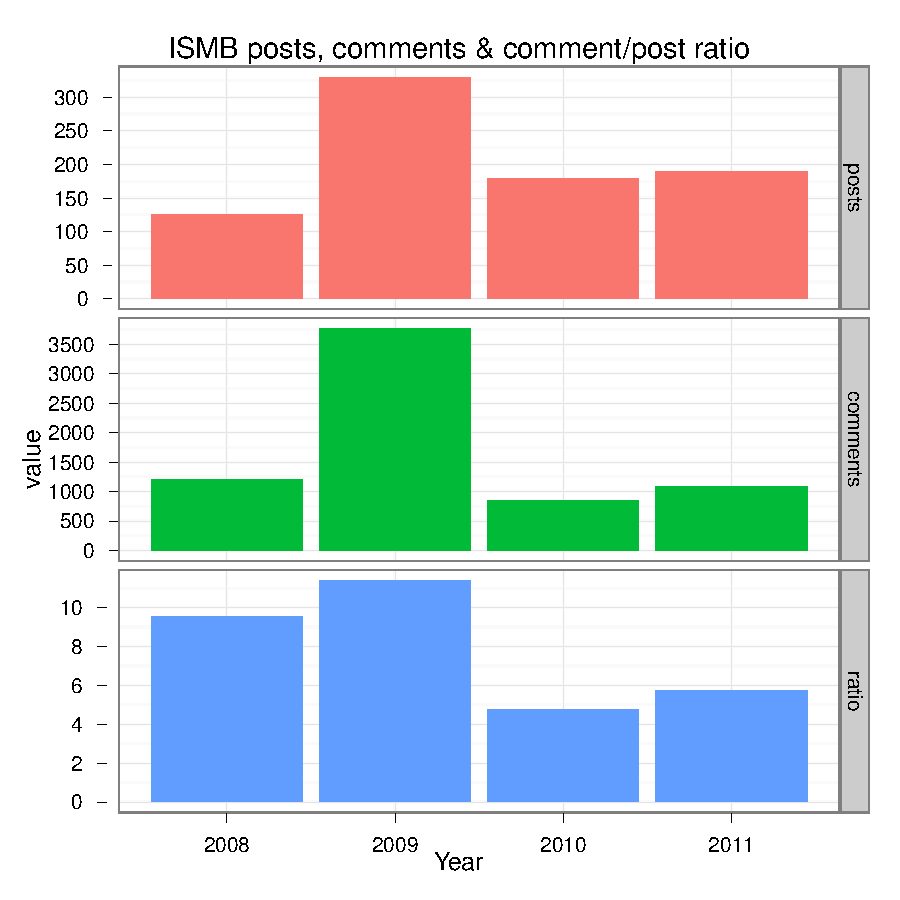
\includegraphics{ismb-004}
\end{center}

\section{Participants who commented}

\begin{center}
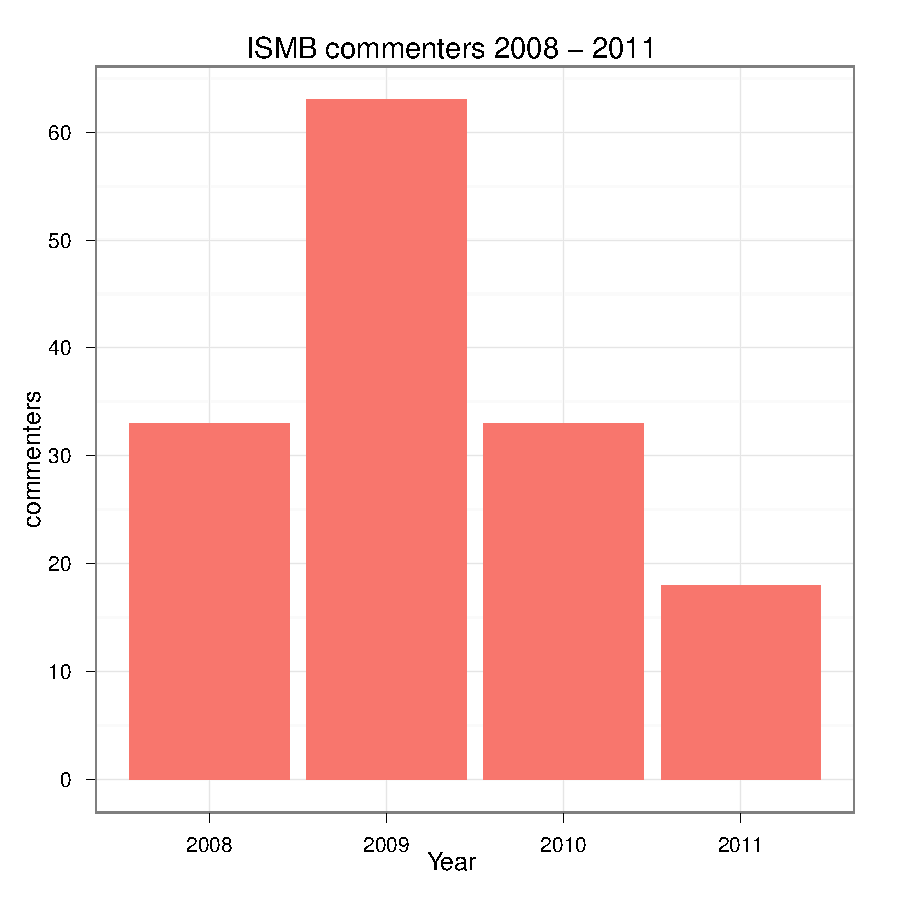
\includegraphics{ismb-006}
\end{center}

\section{Posts with/without comments}

\begin{center}
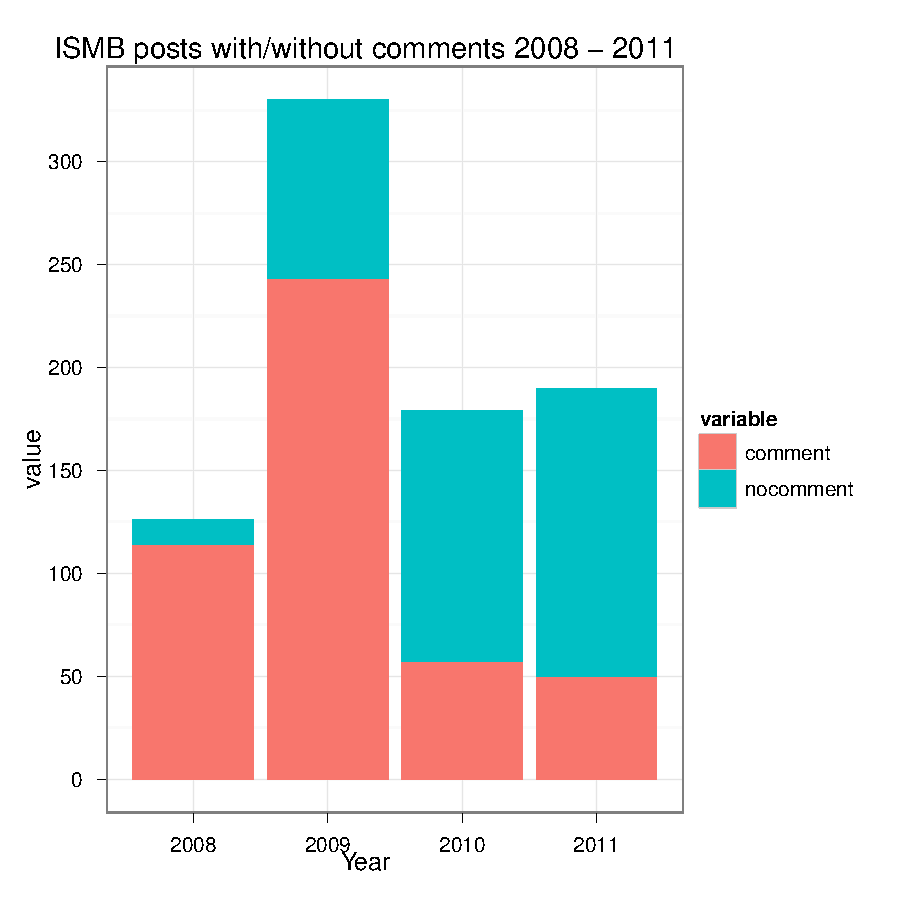
\includegraphics{ismb-008}
\end{center}

\section{Comments per post}

\begin{center}
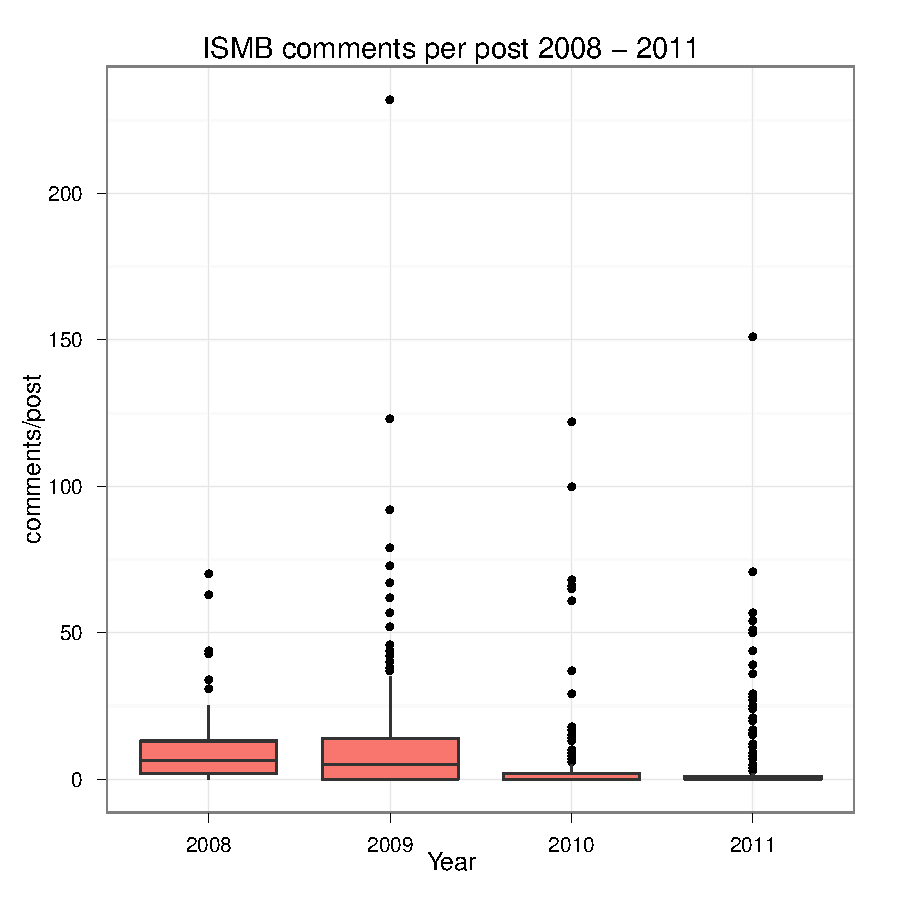
\includegraphics{ismb-010}
\end{center}

\section{Comments per user}

\begin{center}
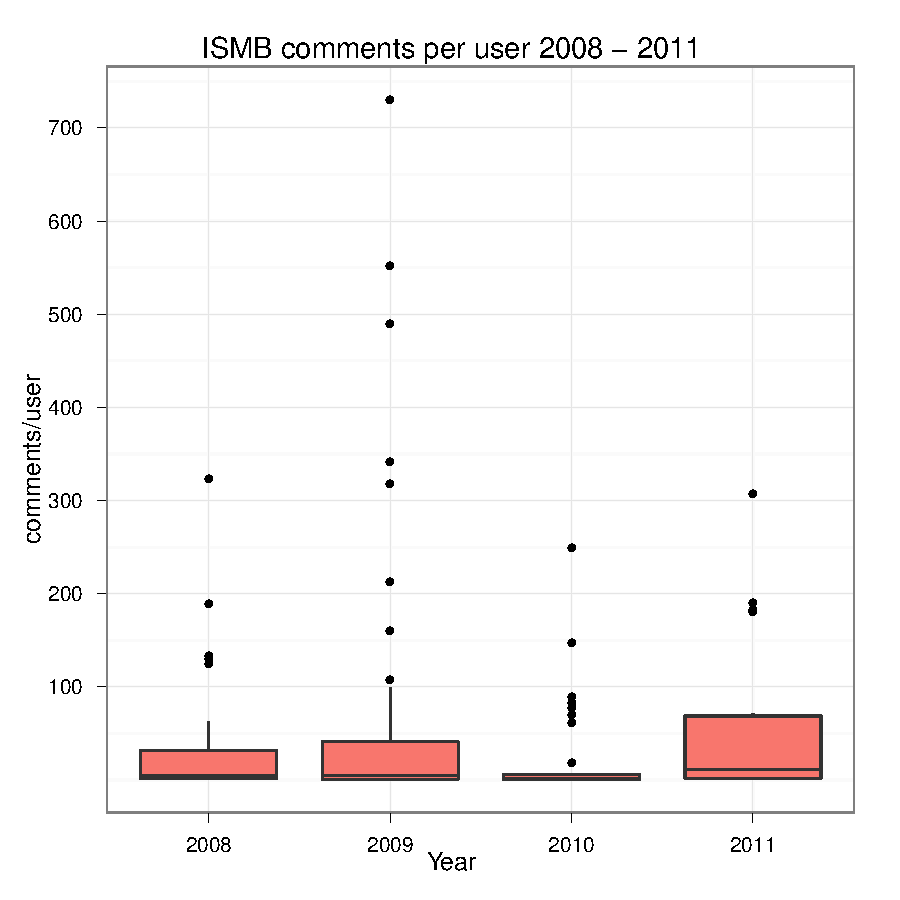
\includegraphics{ismb-012}
\end{center}

\begin{center}
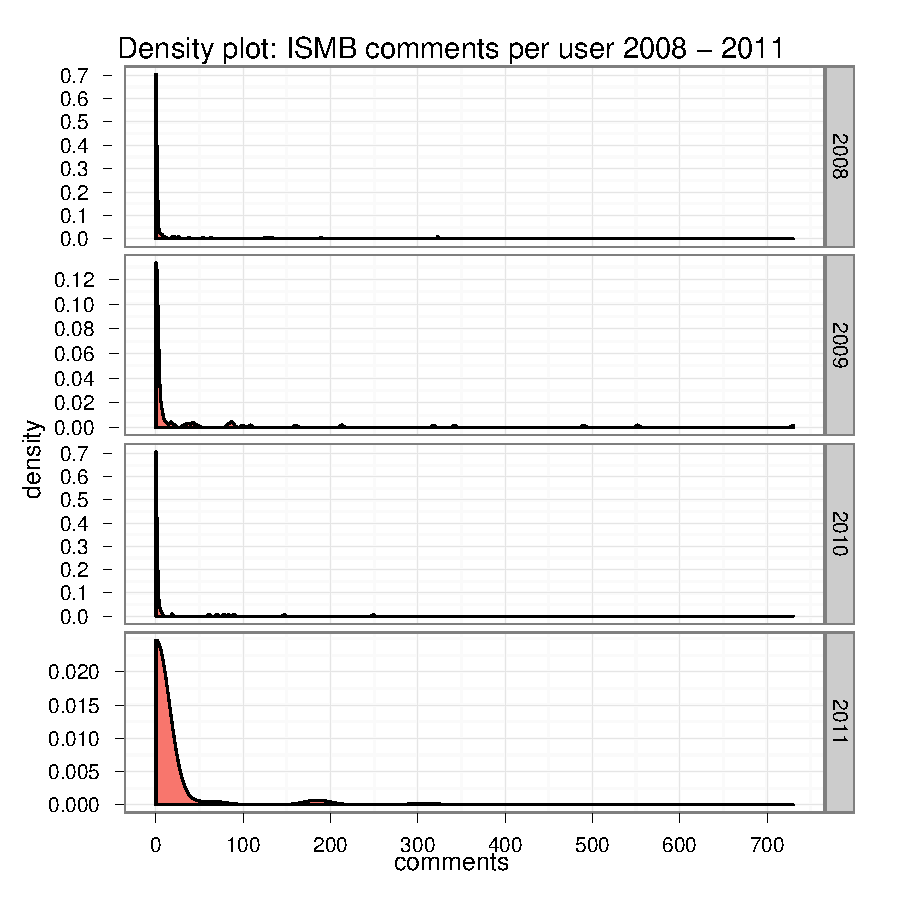
\includegraphics{ismb-013}
\end{center}

\section{Comments timeline}

\begin{center}
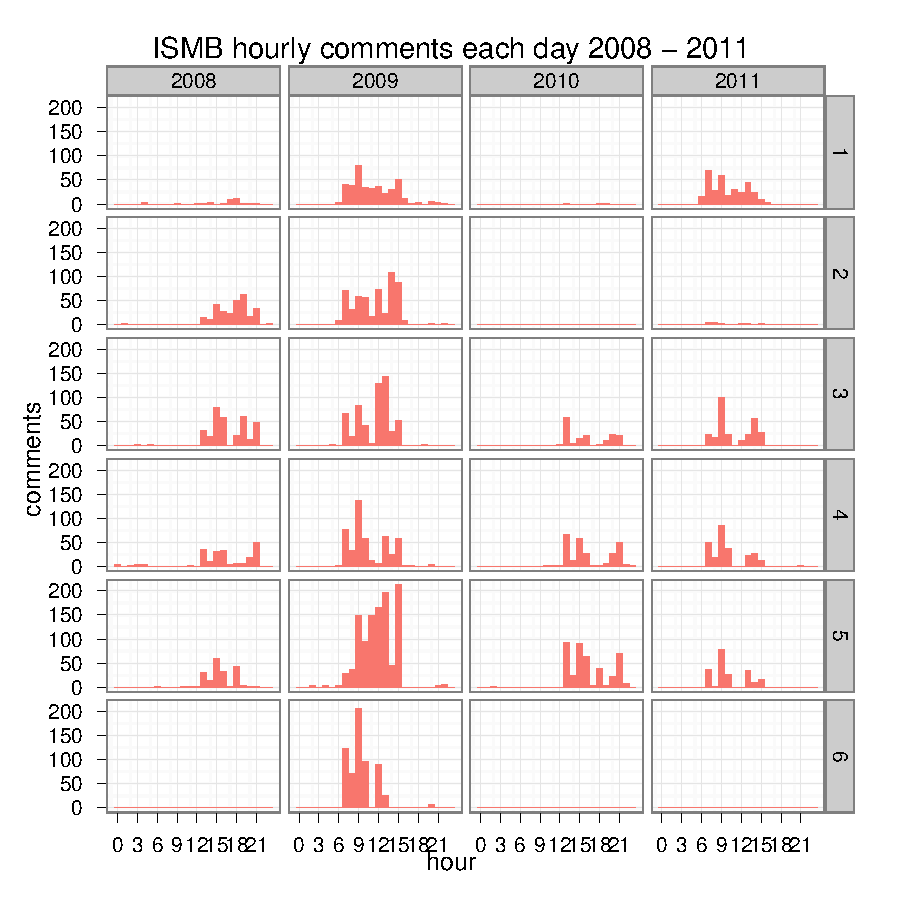
\includegraphics{ismb-015}
\end{center}


\section{Most popular posts}
% latex table generated in R 2.13.0 by xtable 1.5-6 package
% Wed Jul 27 20:30:36 2011
\begin{table}[ht]
\begin{center}
{\small
\begin{tabular}{rlr}
  \hline
year & body & comments \\ 
  \hline
2009 & Keynote: Thomas Lengauer - Chasing the AIDS Virus & 232 \\ 
  2011 & SNP-SIG: Identification and annotation of SNPs in the context of structure, function, and disease & 151 \\ 
  2009 & Keynote: Mathias Uhlen - A global view on protein expression based on the Human Protein Atlas & 123 \\ 
  2010 & PLoS Session on How to Write a Good Paper & 122 \\ 
  2010 & Keynote: David Altshuler - Genomic Variation and the Inherited Basis of Common Disease & 100 \\ 
  2009 & Keynote: Webb  Miller - Bioinformatics Methods to Study Species Extinctions & 92 \\ 
  2009 & Keynote: Daphne Koller - Individual Genetic Variation: From Networks to Mechanisms & 79 \\ 
  2009 & Special Session 6: Regulatory Genome Architecture and Noncoding Mutations in Human Disease & 79 \\ 
  2009 & Birds of a Feather session: Semantic Web-Linked Data, organized by Eric Neumann, in T5 & 73 \\ 
  2011 & Network Biology SIG: On the Analysis and Visualization of Networks in Biology & 71 \\ 
   \hline
\end{tabular}
}
\end{center}
\end{table}
\end{document}
